% Note that the a4paper option is mainly intended so that authors in
% countries using A4 can easily print to A4 and see how their papers will
% look in print - the typesetting of the document will not typically be
% affected with changes in paper size (but the bottom and side margins will).
% Use the testflow package mentioned above to verify correct handling of
% both paper sizes by the user's LaTeX system.
%
% Also note that the "draftcls" or "draftclsnofoot", not "draft", option
% should be used if it is desired that the figures are to be displayed in
% draft mode.
%
\documentclass[10pt,a4paper,conference]{IEEEtran}
\usepackage[brazil]{babel}
\usepackage[utf8]{inputenc}
\usepackage[T1]{fontenc}

\usepackage{graphicx}
\usepackage{amsfonts,amssymb}
\usepackage{hyperref}



% correct bad hyphenation here
\hyphenation{}


\begin{document}
%
% paper title
% can use linebreaks \\ within to get better formatting as desired
\title{Aplicação de análise morfológica para \\segmentação de páginas em imagens de documentos}

%------------------------------------------------------------------------- 
% author names and affiliations
% use a multiple column layout for up to two different
% affiliations

\author{%
    \IEEEauthorblockN{Ricardo de Cillo (aluno) e Nina S. T. Hirata (orientadora)}
    \IEEEauthorblockA{%
        Departamento de Ciência da Computação\\
        Instituto de Matemática e Estatística\\
        Universidade de São Paulo\\
    }
}

% for over three affiliations, or if they all won't fit within the width
% of the page, use this alternative format:
% 
%\author{\IEEEauthorblockN{Michael Shell\IEEEauthorrefmark{1},
%Homer Simpson\IEEEauthorrefmark{2},
%James Kirk\IEEEauthorrefmark{3}, 
%Montgomery Scott\IEEEauthorrefmark{3} and
%Eldon Tyrell\IEEEauthorrefmark{4}}
%\IEEEauthorblockA{\IEEEauthorrefmark{1}School of Electrical and Computer Engineering\\
%Georgia Institute of Technology,
%Atlanta, Georgia 30332--0250\\ Email: see http://www.michaelshell.org/contact.html}
%\IEEEauthorblockA{\IEEEauthorrefmark{2}Twentieth Century Fox, Springfield, USA\\
%Email: homer@thesimpsons.com}
%\IEEEauthorblockA{\IEEEauthorrefmark{3}Starfleet Academy, San Francisco, California 96678-2391\\
%Telephone: (800) 555--1212, Fax: (888) 555--1212}
%\IEEEauthorblockA{\IEEEauthorrefmark{4}Tyrell Inc., 123 Replicant Street, Los Angeles, California 90210--4321}}


%------------------------------------------------------------------------- 
% Special Sibgrapi teaser

%------------------------------------------------------------------------- 



% make the title area
\maketitle


% Wherever Times is specified, Times Roman or Times New Roman may be used. If neither is available on your system, please use the font closest in appearance to Times. Avoid using bit-mapped fonts if possible. True-Type 1 or Open Type fonts are preferred. Please embed symbol fonts, as well, for math, etc.

%==========================================
%==========================================


%==========================================

\section{Introdução}

Uma das aplicações da teoria de visão computacional é a análise de
imagens de documentos, área de pesquisa bastante ativa mesmo sendo
explorada a algumas décadas~\cite{10.1109/ICDAR.2007.207}. Isto se deve a sua importância
prática e a complexidade dos problemas abordados.

O objetivo em análise de documentos é extrair informações sobre o
conteúdo e estrutura de um documento digitalizado. O diagrama
\ref{fig:context1}, adaptado de~\cite{Kasturi_OGorman_Govindaraju_2002},
 mostra os diferentes problemas abordados nesse campo de pesquisa.
\begin{figure*}[htb]
\begin{center}
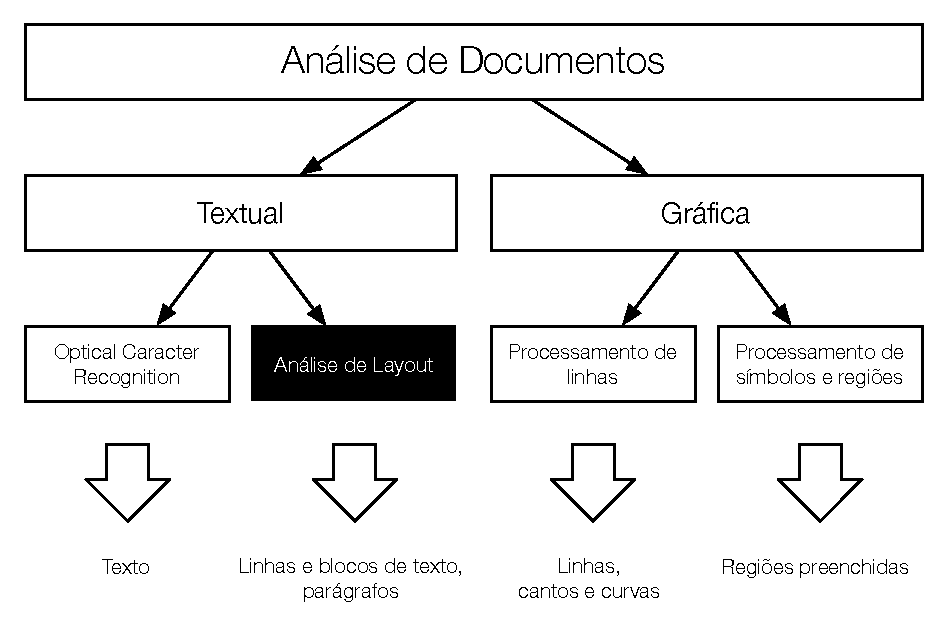
\includegraphics[width=0.7\textwidth]{assets/document_processing_areas_hierarquies.pdf}
\end{center}
\caption{Contextualização do tema do trabalho entre as áreas da
  análise de documentos.}
\label{fig:context1}
\end{figure*}

Uma das etapas envolvidas na análise de layout é a segmentação de
página que consiste na separação e classificação de regiões da
imagem. Diferentes técnicas de processamento e análise de imagens têm
sido propostos e aplicados para tratar esse problema.
O objetivo deste trabalho é investigar a aplicação de operadores
morfológicos~\cite{Serra:1983:IAM:1098652} na segmentação de
páginas. A qualidade da solução obtida será medida e comparada,
segundo os mesmo critérios aplicados à resultados considerados estado
da arte por pesquisadores da área~\cite{10.1109/ICDAR.2007.207}.


\section{Metodologia}

Uma grande diversidade de métodos já foram explorados na solução do
problema de segmentação de
páginas. Em~\cite{Antonacopoulos95representationand} os autores
propõem um método
que observa a distribuição dos espaços em branco em um documento para
classificar a região em texto ou não. Já
em~\cite{Moll07documentcontent} extrai-se características dos pixels e
sua vizinhança, classificando-os e posteriormente agrupando-os em regiões.


\subsection{Treinamento de operadores morfológicos}

Os operadores morfológicos~\cite{Serra:1983:IAM:1098652} são bastante
utilizados na área de visão computacional, para diferentes tipos de
processamento de imagens. A construção de operadores morfológicos
eficazes consiste em geral na combinação sequencial de operadores
simples e pode ser uma tarefa difícil, além de demandar muita
experiência. Portanto, neste trabalho propomos a construção de tais
operadores, para a tarefa de segmentação de páginas, de forma
automática a partir de imagens de treinamento, como descrito em
\cite{Tomita:1996:PrAuMa}.

A figura~\ref{fig:schema_overview} ilustra o esquema geral de
construção de um operador morfológico baseado em treinamento.
\begin{figure*}[htb!]
\begin{center}
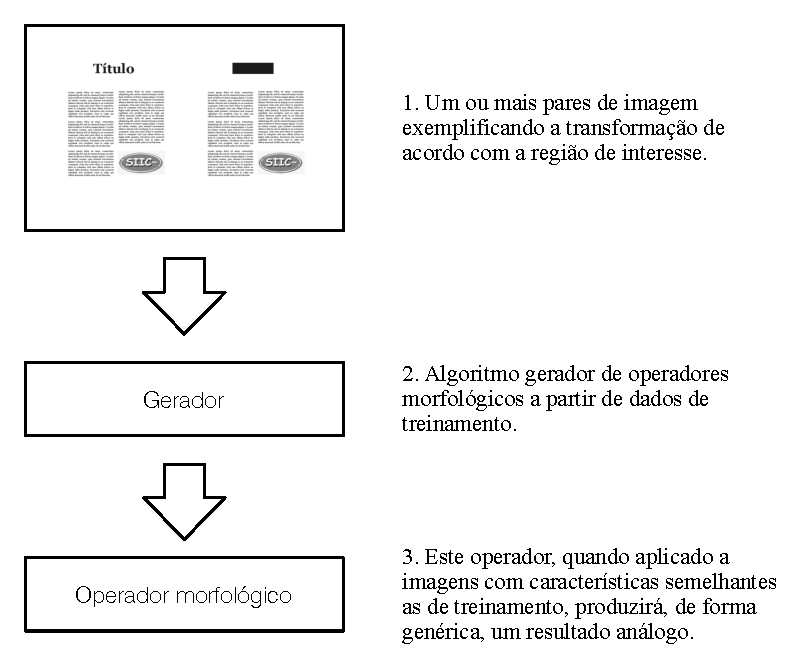
\includegraphics[scale=0.9]{assets/methodology.pdf}
\end{center}
\caption{Visão global do funcionamento.}
\label{fig:schema_overview}
\end{figure*}

As imagens binárias definidas em um certo domínio $E$ (geralmente
$E=\mathbb{Z}^2$) podem ser modeladas por uma função $f: E \to
\{0,1\}$ tal que $f(x)=1$ se e somente se $x$ é um pixel
correspondente a um objeto na imagem (portanto, $f(x)=0$ se $x$
é um pixel do fundo (\emph{background}) da imagem).

O conjunto de todas as imagens binárias definidas em $E$ é denotado
por $\{0,1\}^E$. Desta forma, um operador de imagens binárias é um
mapeamento do tipo $\Psi: \{0,1\}^E \to \{0,1\}^E$. 

Seja $W$ uma janela de observação. Imagens podem ser processadas pixel
a pixel, considerando-se a vizinhança de cada pixel definida pela
janela $W$. Tais processamentos podem ser caracterizados por uma
função do tipo $\psi: \{0,1\}^W \to \{0,1\}$, da seguinte forma
\begin{equation}
[\Psi(f)](x) = \psi(f_{-x}|_W),
\end{equation} 
na qual $f_{-x}|_W$ representa a imagem binária $f$ restrita a $W$ em
torno de $x$. 

% (Esta outra forma de representar $\Psi$ é vantajosa
% pois a cardinalidade do domínio pode ser menor, permitindo implementá-la
% de forma mais eficiente em um algorítmo, correto? Não sei se o leitor
% se atenta para este fato. Talvez valesse a pena escrever?)


Dada uma imagem $f$ a ser processada e a respectiva imagem ideal $I$
esperada como resultado do processamento, o erro de um operador $\Psi$
é caracterizado por
\begin{equation}
MAE\langle \Psi \rangle = E \big[ [\Psi(f)](z) - I(z) \big]\,,
\end{equation}
na qual $E$ denota o valor esperado.
Supondo estacionaridade, o ponto $z$ é arbitrário. Na prática o erro é
calculado tomando-se a média do erro absoluto computado sobre
todos os pixels da imagem.

Portanto, o problema de projetar operadores morfológicos localmente
caracterizados reduz-se ao problema de projetar funçõs binárias do
tipo $\psi: \{0,1\}^W \to \{0,1\}$.
Dado que $P$ é a distribuição conjunta do processo
$(\mathbf{X},\mathbf{y})$ (padrões observados pela janela $W$ e
respectivo valor da imagem de saída para o pixel considerado), pode-se
mostrar que o operador ótimo em relação ao erro MAE é dado por
\begin{equation}
\label{eq:opt}
\psi(X) = \left\{
          \begin{array}{ll}
          1, & \mbox{se $P(X,0)<P(X,1)$,}\\
          0, & \mbox{se $P(X,0)>P(X,1)$,}\\
          1 \mbox{ ou } 0, & \mbox{if $P(X,0)=P(X,1)$.}
          \end{array}
\right.
\end{equation}

Na prática, essas probabilidades não são conhecidas. Portanto, no
processo de aprendizado de operadores, as mesmas são estimadas a partir
de imagens de treinamento (pares de imagens entrada-saída, sendo que
as imagens de saída em geral são geradas editando-se a imagem de
entrada). A partir das probabilidades estimadas, pode-se obter a
decisão ótima de acordo com a equação~\ref{eq:opt}. No entanto, nem
todos os padrões $X$ são observados nas imagens de
treinamento. Portanto, utiliza-se um algoritmo de aprendizado para que
a função característica do operador resultante fique completamente
definida. Frequentemente, a esse processo de atribuir uma
classificação para os padrões não pertencentes ao conjunto de
treinamento é denominado de generalização.

Diferentes algoritmos de aprendizado podem ser
utilizados. Em~\cite{Tomita:1996:PrAuMa}, utiliza-se a minimização de
funções booleanas não especificadas completamente. Maiores detalhes do
método de treinamento podem ser encontrados em~\cite{Nina:2010a}.


\subsection{Avaliação da segmentação}

A fim de comparar de forma objetiva o desempenho do método
desenvolvido, aplicaremos aos resultados o avaliador automático
utilizado na competição internacional de segmentação de página
ICDAR2009 \cite{DBLP:conf/icdar/2009}.

Este avaliador compara os resultados gerados pelo algoritmo a um
resultado manualmente construído. A representação das regiões é feita
com polígonos isotéticos, onde todos os ângulos possuem 90 graus. Esta
geometria é flexível o suficiente para representar regiões complexas e
não apenas áreas retangulares.

% achei desnecessário para um resumo explicar a estrutura de dados utilizada pelo avaliador.

O processo de medição da acurácia leva em consideração as seguintes
relações entre as áreas computadas e esperadas:

\begin{itemize}
	\item intersecção nula,
	\item cobertura total da região esperada,
	\item duas regiões computadas cobrindo apenas uma região esperada,
	\item uma região computada cobrindo duas regiões esperadas, e
	\item região esperada esquecida.
\end{itemize}

Alguns dos erros descritos acima podem receber um peso maior
dependendo do contexto. Agrupar regiões distintas cuja ordem de
leitura seja sequencial, por exemplo, não é considerado um erro.

\section{Resultados esperados}

Alguns resultados publicados atestam a viabilidade do
treinamento de operadores morfológicos na segmentação de
páginas~\cite{HirBarTer:00,Nina:2010a}. No entanto, nesses trabalhos a
segmentação de páginas é apresentada apenas como um exemplo de
possível aplicação, e em geral considerando páginas com estruturas bem
controladas.

Neste trabalho, os experimentos estão sendo realizados com um conjunto
de dados
diversificados~\cite{Antonacopoulos09arealistic}, que simula de forma
mais realista uma situação de aplicação real e não apenas documentos
estruturados de forma mais previsível e controlada. Para o treinamento
do operador morfológico está sendo utilizado o pacote TRIOS
(\emph{TRaining Image Operators from Samples}~\cite{trios:online}),
que é uma versão para Python do software utilizado em trabalhos
anteriores.

Entre os principais desafios enfrentados encontra-se o treinamento de
um operador morfológico que seja capaz de lidar com fontes de
diferentes tipos e tamanhos. Está em investigação também a forma
adequada para as imagens de saída para o treinamento: imagens
consitindo apenas de textos da página de entrada, ou imagens
consistindo do polígono isotético preenchido das regiões de texto.

Finalmente, os resultados obtidos serão comparados com os resultados
esperados (\emph{ground-truth}), segundo a métrica descrita acima.


{\small 
\bibliographystyle{unsrt}	% (uses file "plain.bst")
\bibliography{myrefs}		% expects file "myrefs.bib"
}

%\bibliographystyle{IEEEtran}
%\bibliography{bib_extra/refs}

\end{document}

